\documentclass[12pt]{article}
%%% ========== Package setup ==========
\usepackage{listings}   % Script listing package
\usepackage{wrapfig}    % Wrap Figure or table package
\usepackage{multicol}   % Multicolumn package
\usepackage{pdfpages}   % Include pdf files

%%% ========== Format setup ==========
%% Setup chinese words encoder
\usepackage{xeCJK}
\XeTeXlinebreaklocale "zh"
\XeTeXlinebreakskip = 0pt plus 1pt

%% More word fonts
\usepackage{fontspec}
\setmainfont{Times New Roman}
\renewcommand{\familydefault}{\rmdefault}
\setCJKmainfont{標楷體}

%% Chinese paragraph format
\usepackage{indentfirst}
\setlength{\parindent}{2em}

%% Page margin
\usepackage[a4paper, total={6in,8in}]{geometry}

%%% ========== Document ==========
\begin{document}
\newcommand{\MakeTitlePage}[1]{
\begin{titlepage}
    \begin{center}

        \fontsize{50}{10}
        \selectfont
        Optimal Control

        \vspace{1cm}

        \fontsize{30}{10}
        \selectfont
        Final exam

        \vspace{11cm}

        \begin{tabular}{ r l }
            班級: & 航太四A \\ [10pt]
            姓名: & 吳柏勳 \\ [10pt]
            學號: & 407430635 \\ [10pt]
            座號: & 3 \\ [10pt]
        \end{tabular}

    \end{center}
\end{titlepage}
}
\MakeTitlePage{9}
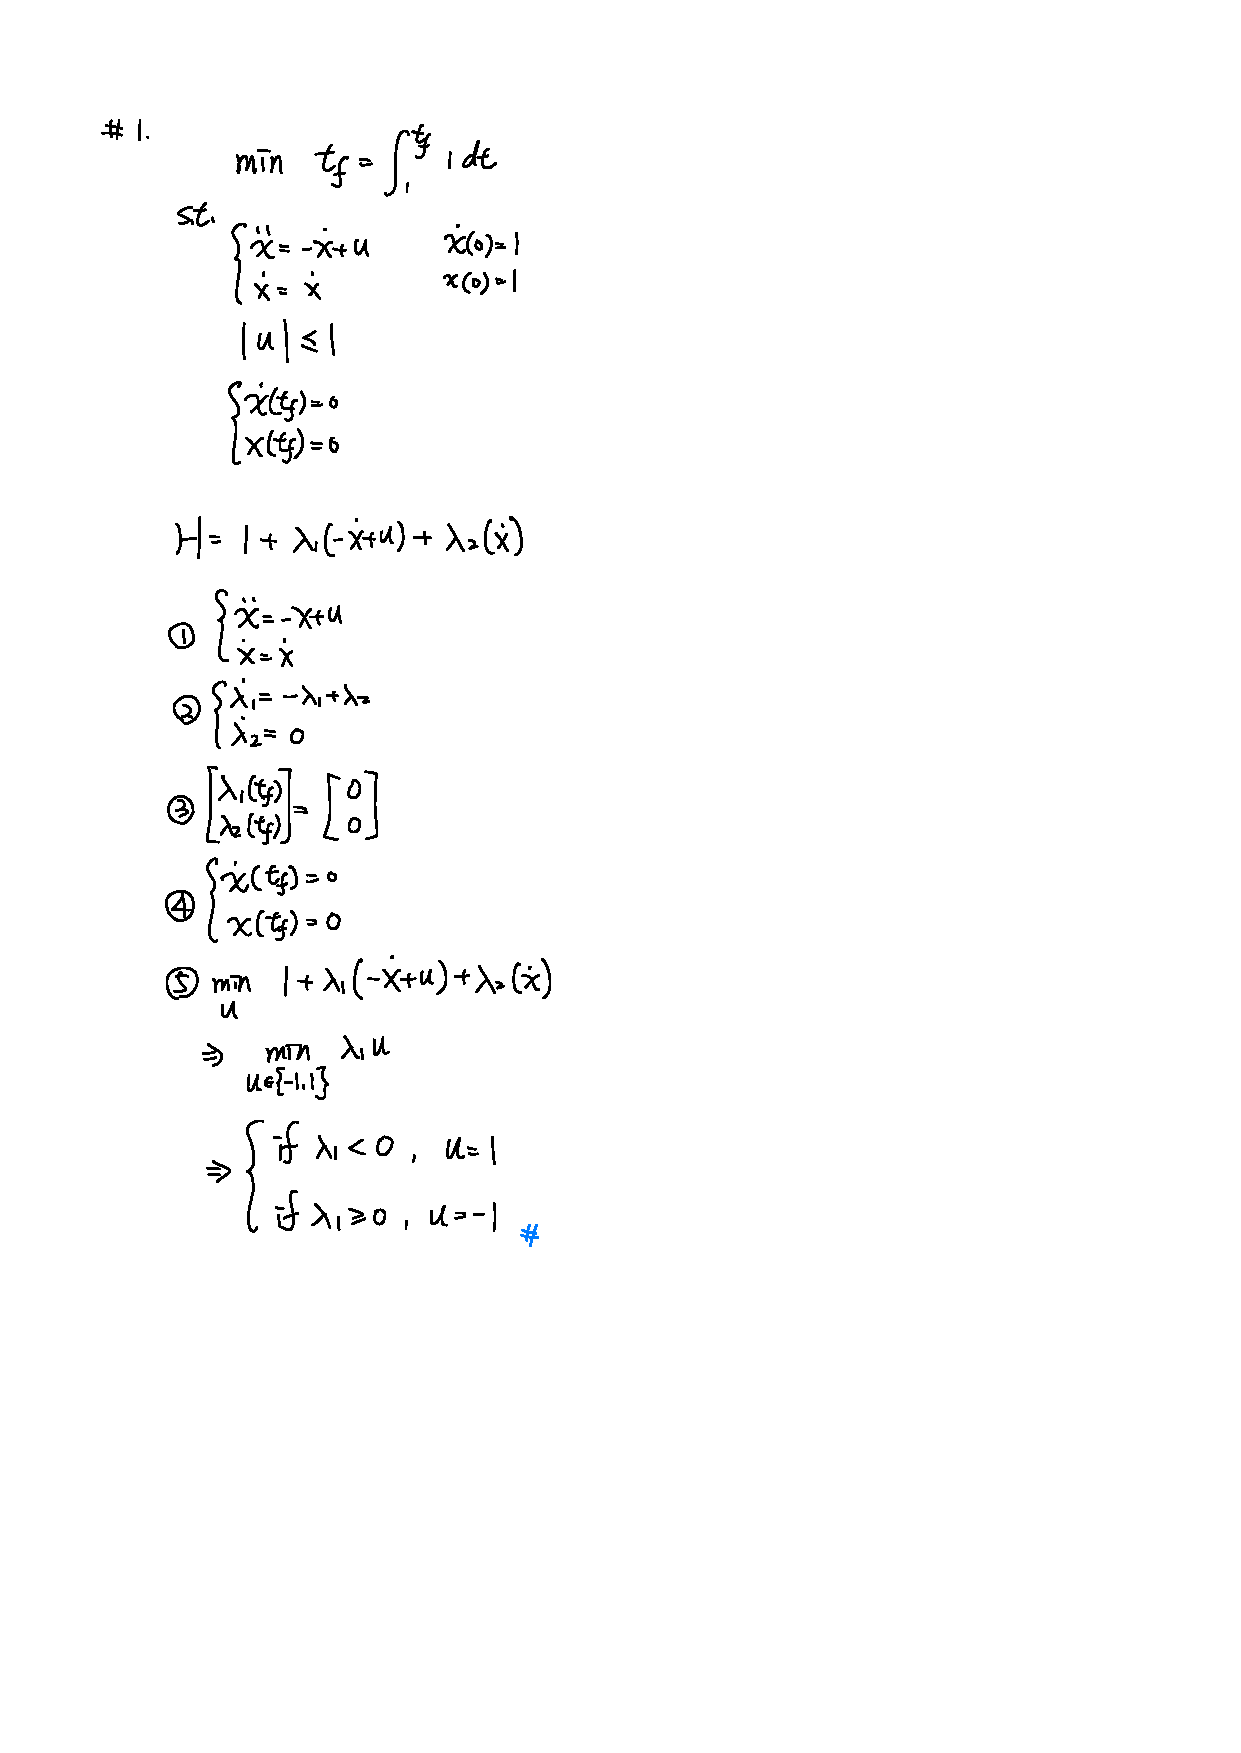
\includepdf[pages=-]{handout.pdf}

\begin{verbatim}
clear;clc;close all
[t, x] = ode45(@ODE, [4.8 0], [0 0 0 0]');

figure()
plot(t, x(:,1), t, x(:,2))
legend("$\dot{x}$", "$x$", 'Interpreter', 'latex')
grid on

function dxdt = ODE(~, x)
    % state define: [x_dot, x, lambda1, lambda2]'

    if x(3)<=0
        u = 1;
    else
        u = -1;
    end

    dxdt = [-x(2)+u
             x(1)
            -x(3)+x(4)
             0];
end
\end{verbatim}

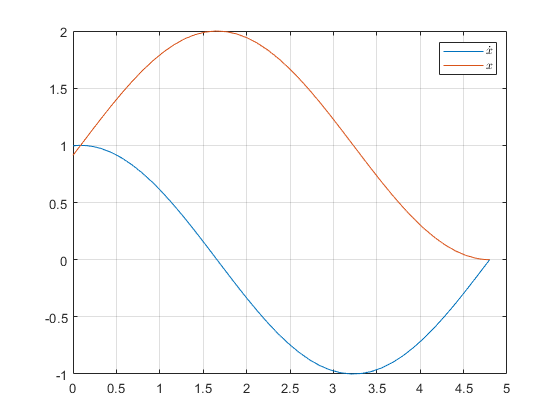
\includegraphics [width=4in]{HW9_01.png}



\end{document}

